% 第 6 周交付物:模型训练调参与最终对比报告(中文版) —— 编译方式:XeLaTeX
\documentclass[11pt]{ctexart}
\usepackage[a4paper, margin=2.4cm]{geometry}
\usepackage{amsmath}
\usepackage{booktabs}
\usepackage{graphicx}
\usepackage[hidelinks]{hyperref}
\usepackage{enumitem}
\setlist{nosep}

\title{\textbf{模型训练、调参与最终对比报告}\\
\large Advanced Chooser Option Pricing Model --- 第 6 周交付物}
\author{佟铸城 (Zhucheng Tong)}
\date{2026 年 8 月}

\begin{document}
\maketitle

\section{评估协议}
\begin{enumerate}
  \item \textbf{walk-forward 滚动重训}:每 63 个交易日重训一次,训练集为该时点之前的全部可用数据(保持 252 行净化,训练标签的未来窗口不越过预测区块);
  \item \textbf{调参只用验证集}:各模型超参数以验证窗(2023-06 至 2024-03)的 walk-forward 定价 MAE 为准则选择(审计断言保证选择日志中不含任何测试信息);
  \item \textbf{测试集只开封一次}:2024-03 至 2024-12 共 198 个交易日,调参定型后一次性评估,8 指标 + 加权综合分(参照 = 同期 EWMA 基线)+ 四种权重方案敏感性;
  \item 特征修正:利率水平特征替换为相对其滚动一年均值的偏离(\texttt{r\_1y\_dev}),消除第 5 周树模型的分布外叶节点问题;全部目标锚定化(路线 A:$\ln(\sigma/\sigma_{EWMA})$;路线 B:$\ln(P/P_{EWMA})$);MLP 加输入裁剪鲁棒化。
\end{enumerate}

\section{调参结果(验证集)}
\begin{center}
\small
\begin{tabular}{lll}
\toprule
\textbf{模型} & \textbf{选中超参数} & \textbf{验证 MAE(\$)} \\
\midrule
A: Ridge & $\alpha=10$ & 10.77 \\
A: RandomForest & max\_depth=4 & 20.35 \\
A: GBDT & lr=0.03, 200 轮 & 24.17 \\
A: LSTM & 固定配置(hidden 32) & \textbf{2.82} \\
B: Ridge & $\alpha=10$ & 11.09 \\
B: GBDT & lr=0.05, 300 轮 & 23.33 \\
B: MLP(鲁棒化) & (64,32) & 12.12 \\
\bottomrule
\end{tabular}
\end{center}
按协议,验证集最优为 \textbf{LSTM}(MAE 2.82)。

\section{测试集最终结果(开封一次)}
\begin{center}
\small
\begin{tabular}{lrrrrrrr}
\toprule
& \textbf{MAE} & \textbf{RMSE} & \textbf{Bias} & \textbf{P95} & \textbf{$R^2$} & \textbf{Hit10} & \textbf{综合分} \\
\midrule
\textbf{EWMA 基线} & \textbf{8.51} & --- & $-3.4$ & --- & $-34.8$ & \textbf{26.8\%} & \textbf{1.000} \\
B: MLP(鲁棒化) & 14.75 & 18.86 & $+14.3$ & 40.4 & $-104.8$ & 13.6\% & 2.020 \\
A: LSTM(验证集冠军) & 17.07 & 23.80 & $+16.6$ & 53.9 & $-167.5$ & 13.6\% & 2.492 \\
B: GBDT & 20.45 & 22.27 & $+20.4$ & 33.3 & $-146.5$ & 10.6\% & 2.564 \\
A: GBDT & 20.67 & 22.47 & $+20.6$ & 33.0 & $-149.1$ & 10.6\% & 2.593 \\
A: RandomForest & 21.95 & 23.81 & $+21.0$ & 35.2 & $-167.6$ & 6.1\% & 2.756 \\
A: Ridge & 20.71 & 24.91 & $+20.5$ & 47.9 & $-183.6$ & 8.6\% & 2.783 \\
B: Ridge & 21.02 & 25.24 & $+20.8$ & 48.6 & $-188.4$ & 6.6\% & 2.831 \\
\bottomrule
\end{tabular}
\end{center}

\textbf{结论(负结果,如实报告):在严格的样本外协议下,没有任何 ML 配置击败 EWMA 基线};四种权重方案下的综合分第一名均为 EWMA。验证集冠军 LSTM(2.82)在测试集上劣化到 17.07——教科书式的\textbf{验证集过拟合}实例。

\begin{figure}[h!]
\centering
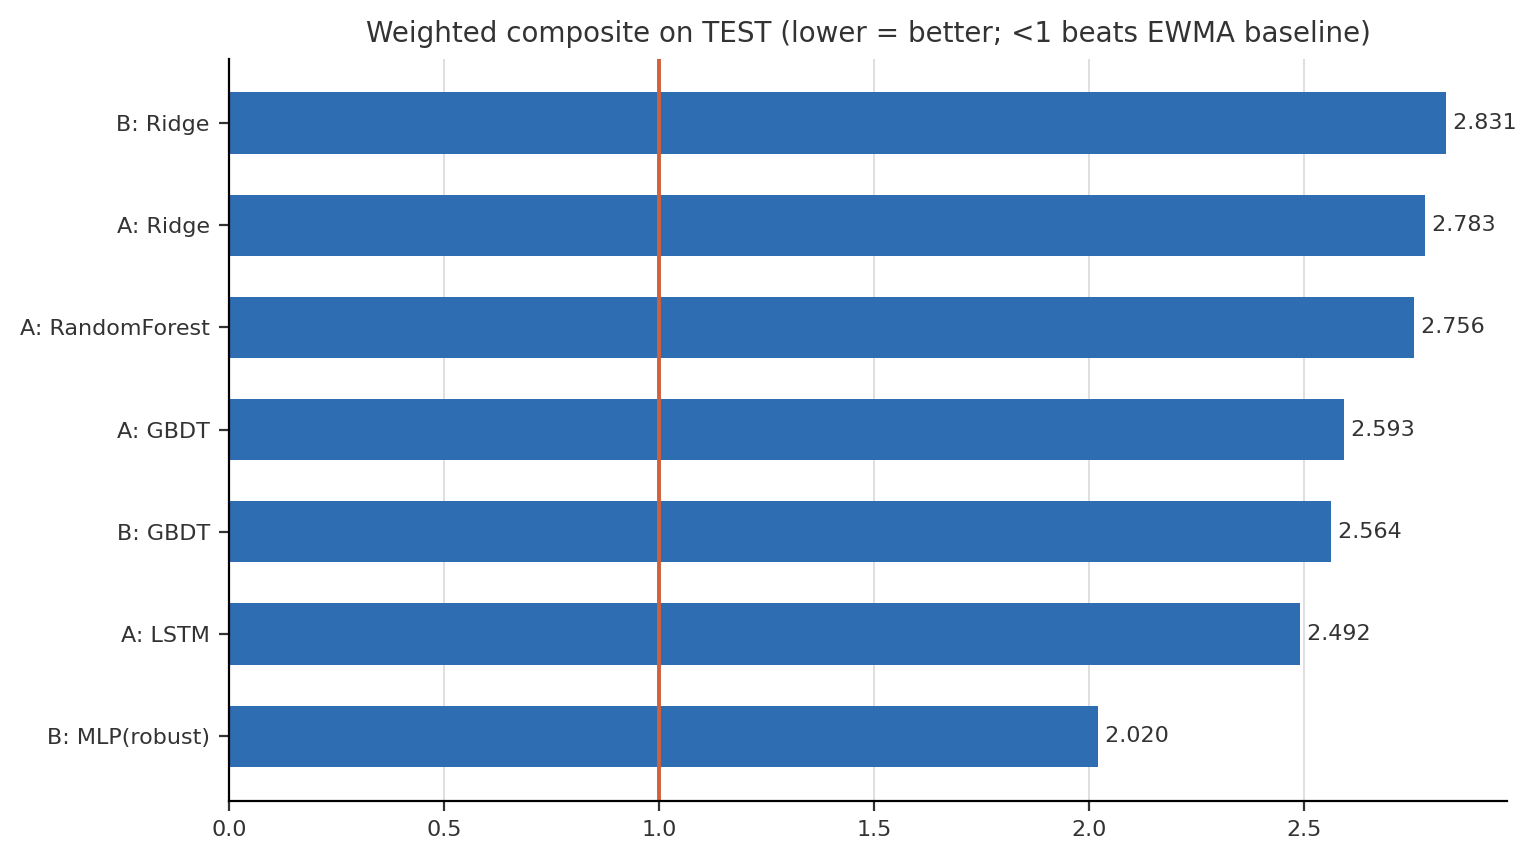
\includegraphics[width=0.78\textwidth]{figures/test_composite.png}
\caption{测试集综合分(所有 ML 模型 $>1$,EWMA 基线胜出)}
\end{figure}

\section{归因分析:为什么 ML 没能赢}
\begin{enumerate}
  \item \textbf{训练数据只覆盖约一个完整波动率周期}:锚定比率目标 $\ln(\sigma_{oracle}/\sigma_{EWMA})$ 有强烈的低频状态自相关(COVID 前为正、2022--23 为负、2024 复为正),664--1050 个高度重叠的训练样本实际上只包含一次半状态轮换——模型学到的是``上一个状态'',而不是可泛化的修正规律;
  \item \textbf{测试标签被不可预见事件污染}:测试期(2024-03 至 2024-12)每一天的标签窗口都覆盖 2025 年 4 月的关税崩盘,真实锚定比率均值 $+0.14$ 的主要来源是这次跳变——与第 4 周``2019 尾段误差''同构,任何回望方法(包括 ML)都不可能预测它;EWMA 之所以获胜,是因为它\textbf{不试图预测};
  \item \textbf{第 5 周验证集胜利的再审视(事后诊断,未用于选择)}:开封后补做的诊断显示,W5 冠军配置(含利率水平特征的一次性训练 Ridge)在 walk-forward 协议下验证 MAE 仅 7.9--8.0(一次性训练时为 3.90),测试 9.25--10.07,同样不敌基线——W5 的胜利部分来自``训练分布恰好偏向正比率''与验证期需求的巧合。结论的教训:\textbf{单一验证窗的胜利不构成部署证据}。
\end{enumerate}

\section{SHAP 可解释性(部署版 GBDT)}
\begin{figure}[h!]
\centering
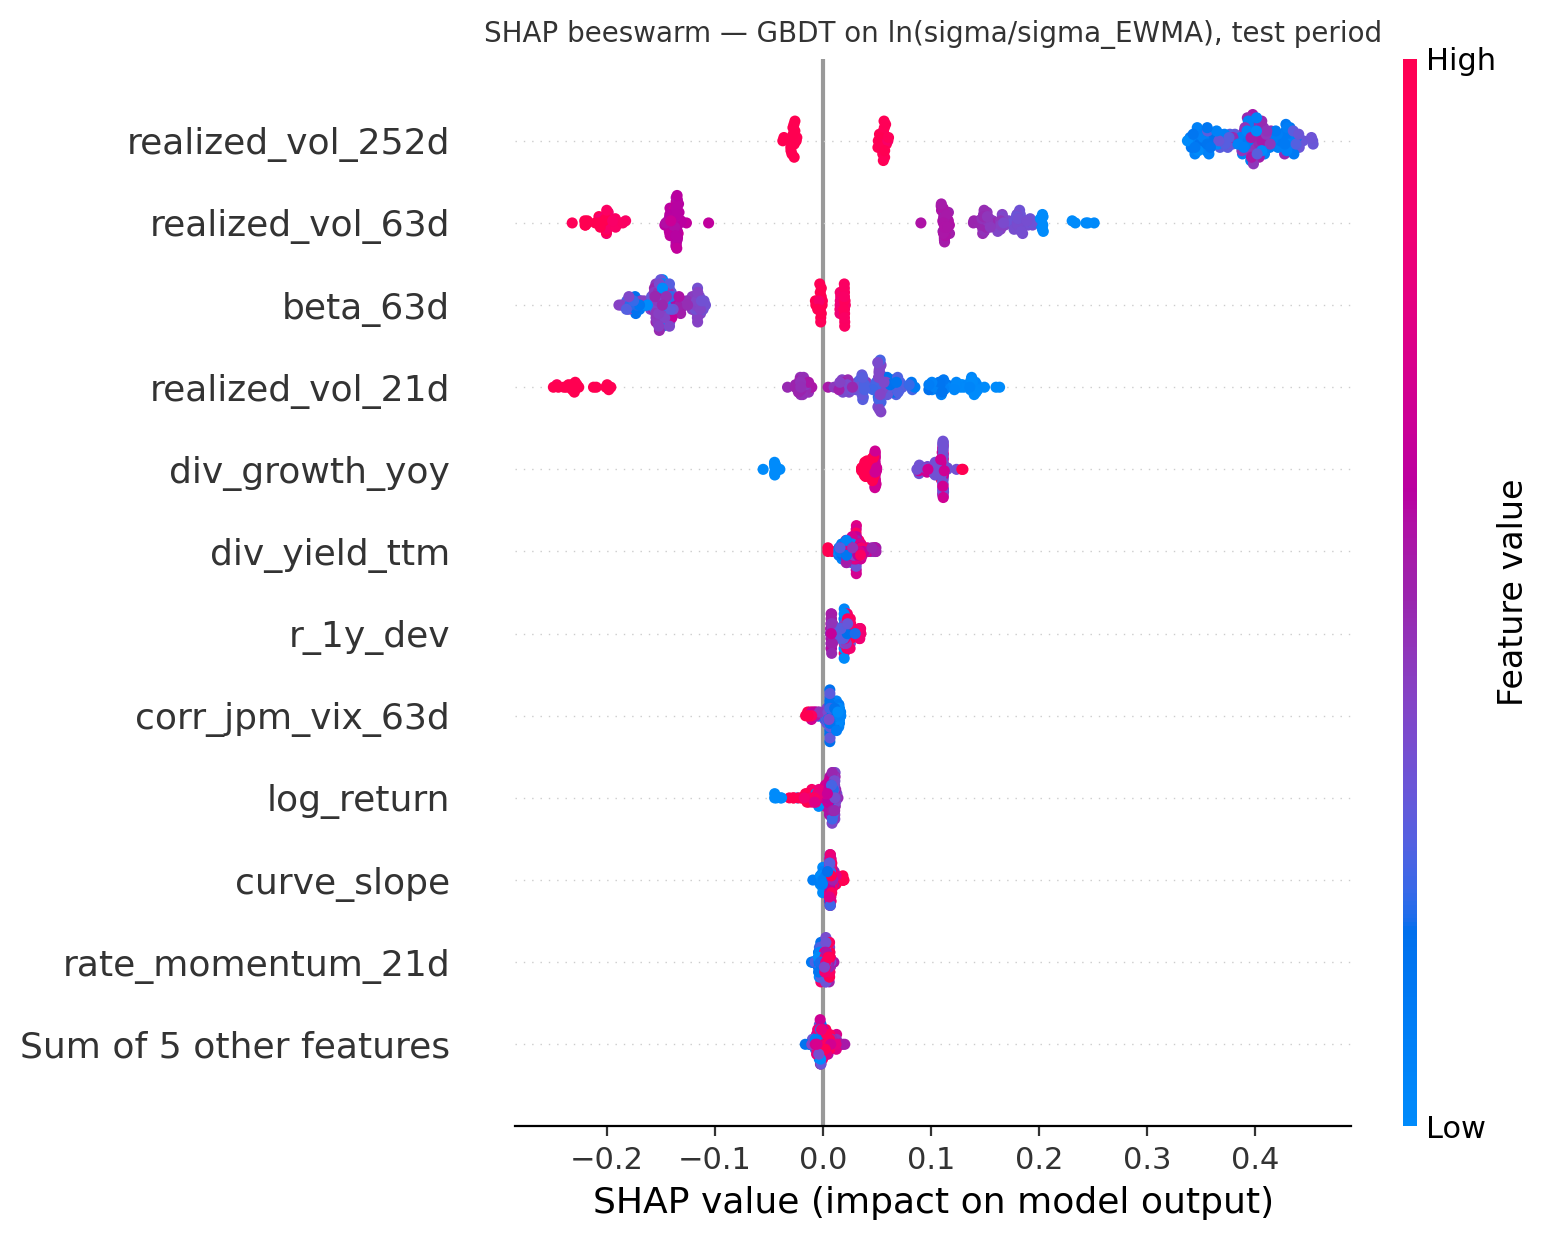
\includegraphics[width=0.72\textwidth]{figures/shap_beeswarm.png}
\caption{SHAP beeswarm(路线 A 锚定目标,测试期)}
\end{figure}
头部特征:\texttt{realized\_vol\_252d}(0.326)、\texttt{realized\_vol\_63d}(0.162)、\texttt{beta\_63d}(0.120)、\texttt{realized\_vol\_21d}(0.081)、\texttt{div\_growth\_yoy}(0.076)。与第 2 周互信息口径一致(长窗口波动率主导),方向上:当前波动率越低,模型越倾向预测正修正(均值回复逻辑)——模型学到的规律本身合理,失败在于该规律的\textbf{幅度}无法从一个周期的数据中稳定标定。

\section{对第 7--8 周工具的决策}
双定价按如下方式落地:\textbf{主定价 = EWMA 锚定 BSM}(全程测试中最稳健);\textbf{ML 修正价作为参考显示},附明确的``样本外未证优''警示与置信说明。诚实的负结果也是可交付的研究结论:它界定了在当前数据规模下 ML 增强的适用边界,并指明改进条件——更长的多周期历史、或引入个股期权隐含波动率数据(替代 VIX 代理)。

\section{可复现性}
全流程固定种子,重跑逐位一致;审计六项(walk-forward 净化、调参日志纯净性、确定性、综合分重算、SHAP 覆盖、解码防护)见 \texttt{analysis/week6/01\_final\_evaluation.py};部署模型 \texttt{models/final\_*.joblib};一键复现 \texttt{python -m src.analysis\_w6}。
\end{document}
